\documentclass[12pt]{article}
\usepackage[utf8]{inputenc}
\usepackage{amsmath}
\usepackage{amssymb}
\usepackage{graphicx}
\usepackage{algpseudocode}
\usepackage{comment}

\graphicspath{ {./} }

\newcommand{\rectres}[1]{
\begin{center}
\begin{tabular}{ |c| }
\hline\\
#1\\
\\
\hline
\end{tabular}
\end{center}
}

\newcommand{\qed}{\hfill$\blacksquare$}

\title{Introduction to AI - 236501\\HW3}
\author{Yair Nahum 034462796\\and\\Hala Awwad 209419134 }

\begin{document}

\maketitle

%\tableofcontents{}

\section*{MDP}

\subsection*{A}

\subsubsection*{A.1.a}

In order to work with our R(s) instead of R(s,a,s') one can define the following:
$$\tilde R(s_t=s) = \mathbb {E}_{s'\in S, a\in A(s)}[R(s_{t+1}=s',a_t=a|s_t=s]=$$
$$= \sum_{s'\in S} \sum_{a\in A(s)} P(s_{t+1}=s',a_t=a|s_t=s) R(s_t=s,a_t=a,s_{t+1}=s') = $$
$$= \sum_{s'\in S} \sum_{a\in A(s)} P(s_{t+1}=s'|a_t=a,s_t=s)\pi(a_t=a|s_t=s) R(s_t=s,a_t=a,s_{t+1}=s') = $$
$$= \sum_{a\in A(s)} \pi(a_t=a|s_t=s) \sum_{s'\in S} P(s_{t+1}=s'|a_t=a,s_t=s) R(s_t=s,a_t=a,s_{t+1}=s') = $$

Thus, the value function on states $s\in S$ with some given policy $\pi(a|s)$ (probability to make an action $a$ when we're in s) is defined recursively by:

$$V^{\pi}(s) = \sum_{a\in A(s)} \pi(a|s) \sum_{s'\in S} P(s'|s,a) [R(s,a,s') + \gamma V(s')]$$

In case we have a deterministic given policy, we can write it as:

$$V^{\pi}(s) = \sum_{s'\in S} P(s'|s,\pi(s)) [R(s,\pi(s),s') + \gamma V(s')]$$

(We assumed a stationary policy and dynamics so we didn't subscript/relate to time on probabilities.)

\subsubsection*{A.1.b}

The Bellman operator:

$$V^*(s) = \max_{a\in A(s)}Q^*(s,a) = \max_{a\in A(s)} \sum_{s'\in S} P(s'|s,a) [R(s,a,s') + \gamma V^*(s')]$$

\subsubsection*{A.1.c}

Value Iteration (VI):\\

\begin{enumerate}
  \item Start with any initial value function (zero or random) $V_0(s),\quad \forall s\in S$.
  \item Compute recursively, for $n = 0,1,2, \ldots $ umtil stopping rule is met (see next the stopping rule details:
          \[V_{n + 1}(s) = \max_{a\in A(s)} \sum_{s' \in S} P(s'|s,a)[R(s,a,s') + \gamma V_n(s')], \quad \forall s \in S\]
   \item Extract optimal policy from optimal value by:
   \[\pi(s) \in arg\max_{a\in A(s)} \sum_{s' \in S} P(s'|s,a)[R(s,a,s') + \gamma V^*(s')], \quad \forall s \in S\]
\end{enumerate}
Notes:\\
1. Stopping rule to obtain a required accuracy.\\
  If $$||V_{n+1}-V_{n}||_\infty < \epsilon \cdot \frac{1-\gamma}{\gamma}$$ then $$||V_{n+1} -
V^{*}||_\infty \leq \epsilon$$\\
(this is a theorem that can be proved as done in tutorials)\\
2. For a fixed policy value iteration, the recursive computation is changed to have $\pi(s)$ instead of $a$
$$V^{\pi}_{n + 1}(s) = \sum_{s' \in S} P(s'|s,\pi(s))[R(s,\pi(s),s') + \gamma V^{\pi}_n(s')], \quad \forall s \in S$$
This can be solved also by linear system of equations solver as these are linear equations (usually when the state space is not too big)\\

When $\gamma=1$ VI is not guaranteed to converge unless there are absorbing/goal states ($s\in S_G$ no action to transition out from it) that we can get to with probability 1 eventually ( This is known as episodic MDPs or Stochastic Shortest Path problems).

\subsubsection*{A.1.d}

Policy Iteration (PI):\\
PI consists of 2 main parts: Policy evaluation and Policy improvement.

\begin{enumerate}
\item Select some stationary policy $\pi_0$.
\item For $k = 0,1,2, \ldots $ until stopping rule is met (see next the stopping rule details:
\begin{enumerate}
\item Policy Evaluation: compute $V^{\pi_k}$ by fixed policy VI or by solving linear system of equations:\\
$$V^{\pi_k}_{n + 1}(s) = \sum_{s' \in S} P(s'|s,\pi_k(s))[R(s,\pi_k(s),s') + \gamma V^{\pi_k}_n(s')], \quad \forall s \in S$$
Or:\\
$$V^{\pi_k} = (I - \gamma P^{\pi_k})^{-1} P^{\pi_k}R^{\pi_k}$$
(at the last closed solution there is the $R^{\pi_k}$ which corresponds to the vector of rewards $R(s,\pi_k(s),s')$ multiplied by the transition probabilities matrix for expectancy)
\item Policy Improvement: compute $\pi_{k+1}$, a greedy policy with respect to $V^{\pi_k}$:
$$\pi_{k+1}(s) \in arg\max_{a\in A(s)} \sum_{s' \in S} P(s'|s,a)[R(s,a,s') + \gamma V^{\pi_k}(s')], \quad \forall s \in S$$
\item Stop if $\pi_{k+1} = \pi_{k}$
\end{enumerate}
\end{enumerate}

When $\gamma=1$ PI is not guaranteed to converge unless there are absorbing/goal states ($s\in S_G$ no action to transition out from it) that we can get to with probability 1 eventually ( This is known as episodic MDPs or Stochastic Shortest Path problems).

\subsubsection*{A.1.e}

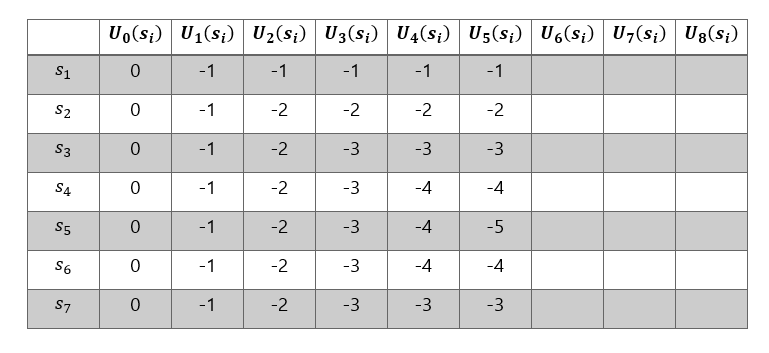
\includegraphics[]{hw3/plots/A_5.PNG}

\subsubsection*{A.1.f}

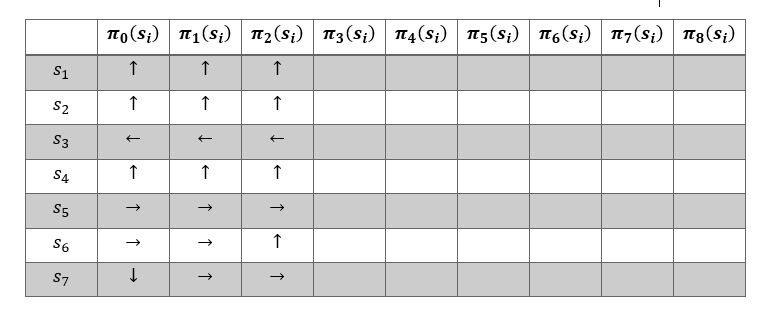
\includegraphics[]{hw3/plots/A_6.PNG}

\subsection*{B}
Wet part code intro. nothing to do.

\subsection*{C}
Wet part in code.

\section*{Learning Introduction}

\subsection*{A}
Wet part code intro. nothing to do.

\subsection*{B}
\subsubsection*{B.1}
\subsubsubsection{B.1.a.}
The entropy $H(Passed)$:
$$H(Passed)= -[\frac{2}{6}\log_2(\frac{2}{6}) + \frac{4}{6}\log_2\frac{4}{6}] = -[\frac{1}{3}(\log_21- \log_23) + \frac{2}{3}(\log_22 - \log_23)]=$$ 
$$-[\frac{2}{3} - \log_23] = \log_23 - \frac{2}{3} \Rightarrow$$
\rectres{$H(Passed)=\log_23 - \frac{2}{3}$}
\subsubsubsection{B.1.b.}
The entropy $H(Passed|Average)$:
$$H(Passed|Average=Low)= -[\frac{1}{2}\log_2\frac{1}{2} +\frac{1}{2}\log_2\frac{1}{2}] = 1$$ 
$$H(Passed|Average=Medium)= -[\frac{1}{2}\log_2\frac{1}{2} +\frac{1}{2}\log_2\frac{1}{2}] = 1$$ 
$$H(Passed|Average=High)= -[1\log_21 + 0\log_20] = 0$$ 
The weighted entropy:
$$H(Passed|Average)=\sum_{i=1}^3\frac{|E_i|}{|E|}entropy(E_i)=$$ $$=\frac{2}{6}H(Passed|Average=Low) + \frac{2}{6}H(Passed|Average=Medium)+$$
$$+\frac{2}{6}H(Passed|Average=High)=\frac{2}{3}\Rightarrow$$
\rectres{$H(Passed|Average)=\frac{2}{3}$}
\subsubsubsection{B.1.c.}
The entropy $H(Passed|Studied)$:
$$H(Passed|Studied=No)= -[\frac{2}{3}\log_2\frac{2}{3} +\frac{1}{3}\log_2\frac{1}{3}] = \log_23 - \frac{2}{3}$$ 
$$H(Passed|Studied=Yes)= -[1\log_21 + 0\log_20] = 0$$ 
The weighted entropy:
$$H(Passed|Studied)=\frac{3}{6}(\log_23 - \frac{2}{3}) + \frac{3}{6}0= \frac{1}{2}\log_23 - \frac{1}{3}$$ 
\rectres{$H(Passed|Studied)=\frac{1}{2}\log_23 - \frac{1}{3}$}
\subsubsubsection{B.1.d.}

\subsection*{C}
\subsubsection*{C.4}
In code. passed L2/accuracy unit tests.
\subsubsection*{C.5 - ID3 algorithm}
\subsubsubsection{C.5.a.}\\
In code.\\
\\
\subsubsubsection{C.5.b.}\\
basic experiment passed needed accuracy with 94.69\%

\subsubsection*{C.6 - early pruning}
\subsubsubsection{C.6.a.}\\
Pruning improves the generalization and prevent over-fitting. By having leaves with more labels to decide from, we increase our hypothesis statistical significance (law of big numbers) and the variance of our model is reduced.\\
\\
\subsubsubsection{C.6.b.}\\
In code.\\
\\
\subsubsubsection{C.6.c.}\\
\\
\subsubsubsection{C.6.c.i}\\
The plot:\\
\includegraphics[scale=0.5]{hw3/plots/.PNG}
\\
The output:\\
\\
 M value   | Validation Accuracy\\
    35     | 93.03\%\\
    40     | 92.13\%\\
    45     | 91.83\%\\
    50     | 90.96\%\\
    55     | 89.50\%\\
===========================\\
  Best M   | Validation Accuracy\\
    35     | 93.03\%\\
best_m = 35\\
Test Accuracy: 97.35\%\\

\subsubsubsection{C.6.c.ii}\\
\\
\subsubsubsection{C.6.d.}\\
running with the  $best\_m=$ parameter we get better performance over the test data set as the accuracy is now 94.69\%



\end{document}

